% Нумерация страниц
\setcounter{page}{2}

\section*{Задание 1}

При помощи системного вызова fork() создается два процесса-потомка. Для того, чтобы они завершились после процесса-предка, в них вызывается sleep(). При этом процессы-потомки становятся сиротами. Их усыновляет процесс-посредник systemd -user, который является потомком процесса с идентификатором 1.

\begin{center}
    \captionsetup{justification=raggedright,singlelinecheck=off}
    \begin{lstlisting}[label=lst:orphans,caption=Создание процессов-сирот]
#include <stdio.h>
#include <stdlib.h>
#include <sys/types.h>
#include <unistd.h>

#define FORK_ERROR -1
#define ERROR       1
#define OK          0

#define PAUSE       4

#define TASK        "\n<<<<< Task 1 : Creating orphan processes >>>>>\n\n"


int main(void)
{
    pid_t child_pid1, child_pid2;

    if ((child_pid1 = fork()) == FORK_ERROR)
    {
        perror("\nCan't fork child 1.\n");
        exit(ERROR);
    }
    else if (child_pid1 == 0)
    {
        printf("\nBEFORE: \
                \nChild 1: PID = %d, PPID = %d, GPID = %d.\n", getpid(), getppid(), getpgrp());

        sleep(PAUSE);

        printf("\nAFTER: \
                \nChild 1: PID = %d, PPID = %d, GPID = %d.\n", getpid(), getppid(), getpgrp());

        exit(OK);
    }
    else
    {
        printf("\nParent: PID = %d, GPID = %d, child 1 PID = %d.\n", getpid(), getpgrp(), child_pid1);
    }


    if ((child_pid2 = fork()) == FORK_ERROR)
    {
        perror("\nCan't fork child 2.\n");
        exit(ERROR);
    }
    else if (child_pid2 == 0)
    {
        printf("\nBEFORE: \
                \nChild 2: PID = %d, PPID = %d, GPID = %d.\n", getpid(), getppid(), getpgrp());

        sleep(PAUSE);

        printf("\nAFTER: \
                \nChild 2: PID = %d, PPID = %d, GPID = %d.\n", getpid(), getppid(), getpgrp());

        exit(OK);
    }
    else
    {
        printf("\nParent: PID = %d, GPID = %d, child 2 PID = %d.\n", getpid(), getpgrp(), child_pid2);
    }

    return OK;
}
\end{lstlisting}
\end{center}

\begin{figure}[H]
	\begin{center}
		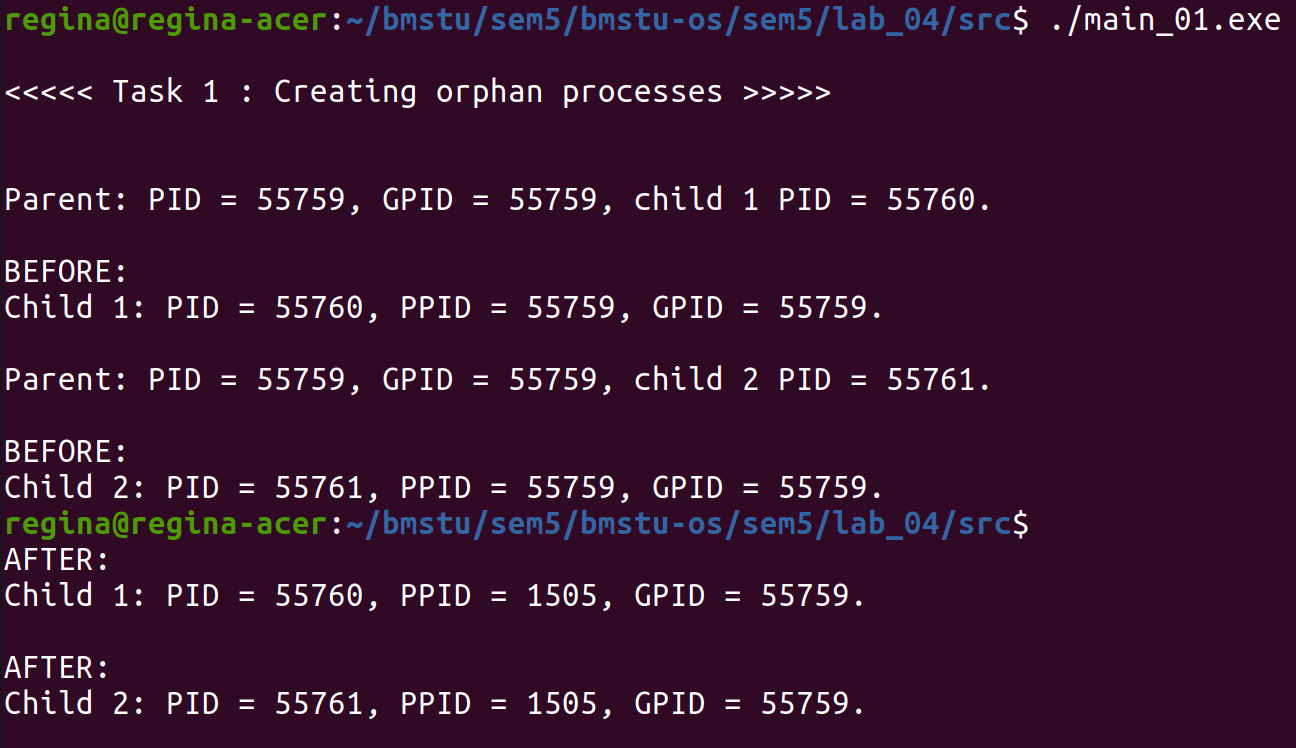
\includegraphics[scale=0.3]{inc/orphans.png}
	\end{center}
	\captionsetup{justification=centering}
	\caption{Демонстрация работы программы}
	\label{img:example}
\end{figure}

\begin{figure}[H]
	\begin{center}
		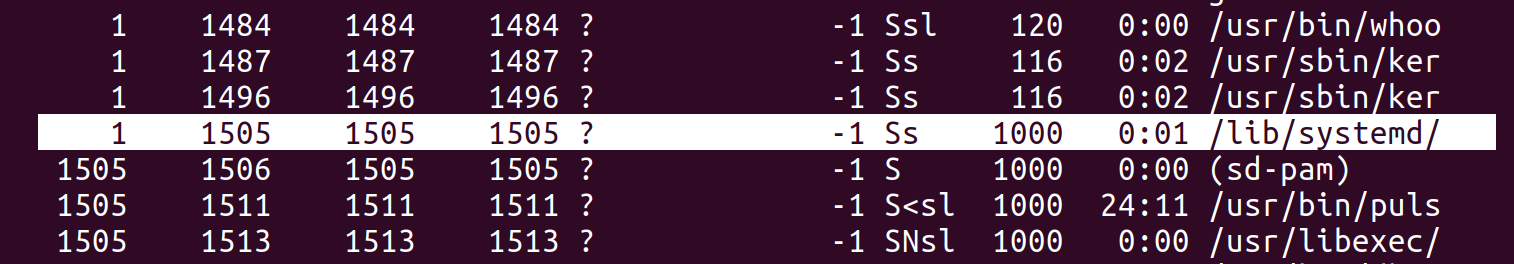
\includegraphics[scale=0.3]{inc/arg.png}
	\end{center}
	\captionsetup{justification=centering}
	\caption{Процесс, усыновивший процессы-сироты}
	\label{img:arg}
\end{figure}

\section*{Задание 2}

Системный вызов wait() блокирует процесс-предок, поэтому он ждет завершения процессов-потомков. Процесс-предок анализирует коды завершения процессов-потомков. 
\clearpage

\begin{center}
    \captionsetup{justification=raggedright,singlelinecheck=off}
    \begin{lstlisting}[label=lst:wait,caption=Системный вызов wait()]
#include <stdio.h>
#include <stdlib.h>
#include <sys/types.h>
#include <sys/wait.h>
#include <unistd.h>

#define FORK_ERROR -1
#define ERROR       1
#define OK          0

#define PAUSE       4

#define TASK        "\n<<<<< Task 2 : Parent is waiting childs with wait() >>>>>\n\n"


void check_status(int status)
{
    if (WIFEXITED(status))
    {
        printf("Child exited correctly with code %d.\n", WEXITSTATUS(status));

        return;
    }
    else if (WIFSIGNALED(status))
    {
        printf("Child exited with non-interceptable signal %d.\n", WTERMSIG(status));

        return;
    }
    else if (WIFSTOPPED(status))
    {
        printf("Child stopped with signal %d.\n", WSTOPSIG(status));

        return;
    }
}


int main(void)
{
    printf(TASK);

    pid_t child_pid1, child_pid2, child_pid;
    int status;

    if ((child_pid1 = fork()) == FORK_ERROR)
    {
        perror("\nCan't fork child 1.\n");
        exit(ERROR);
    }
    else if (child_pid1 == 0)
    {
        printf("\nBEFORE: \
                \nChild 1: PID = %d, PPID = %d, GPID = %d.\n", getpid(), getppid(), getpgrp());

        sleep(PAUSE);

        printf("\nAFTER: \
                \nChild 1: PID = %d, PPID = %d, GPID = %d.\n", getpid(), getppid(), getpgrp());

        exit(OK);
    }
    else
    {
        child_pid = wait(&status);
        printf("\nChild 1 has fihished: PID = %d, status = %d.\n", child_pid, status);

        printf("\nParent: PID = %d, GPID = %d, child 1 PID = %d.\n", getpid(), getpgrp(), child_pid1);
        check_status(status);
    }


    if ((child_pid2 = fork()) == FORK_ERROR)
    {
        perror("\nCan't fork child 2.\n");
        exit(ERROR);
    }
    else if (child_pid2 == 0)
    {
        printf("\n\n\nBEFORE: \
                \nChild 2: PID = %d, PPID = %d, GPID = %d.\n", getpid(), getppid(), getpgrp());

        sleep(PAUSE);

        printf("\nAFTER: \
                \nChild 2: PID = %d, PPID = %d, GPID = %d.\n", getpid(), getppid(), getpgrp());

        exit(OK);
    }
    else
    {
        child_pid = wait(&status);
        printf("\nChild 2 has fihished: PID = %d, status = %d.\n", child_pid, status);

        printf("\nParent: PID = %d, GPID = %d, child 2 PID = %d.\n", getpid(), getpgrp(), child_pid1);
        check_status(status);
    }

    return OK;
}
\end{lstlisting}
\end{center}

\begin{figure}[H]
	\begin{center}
		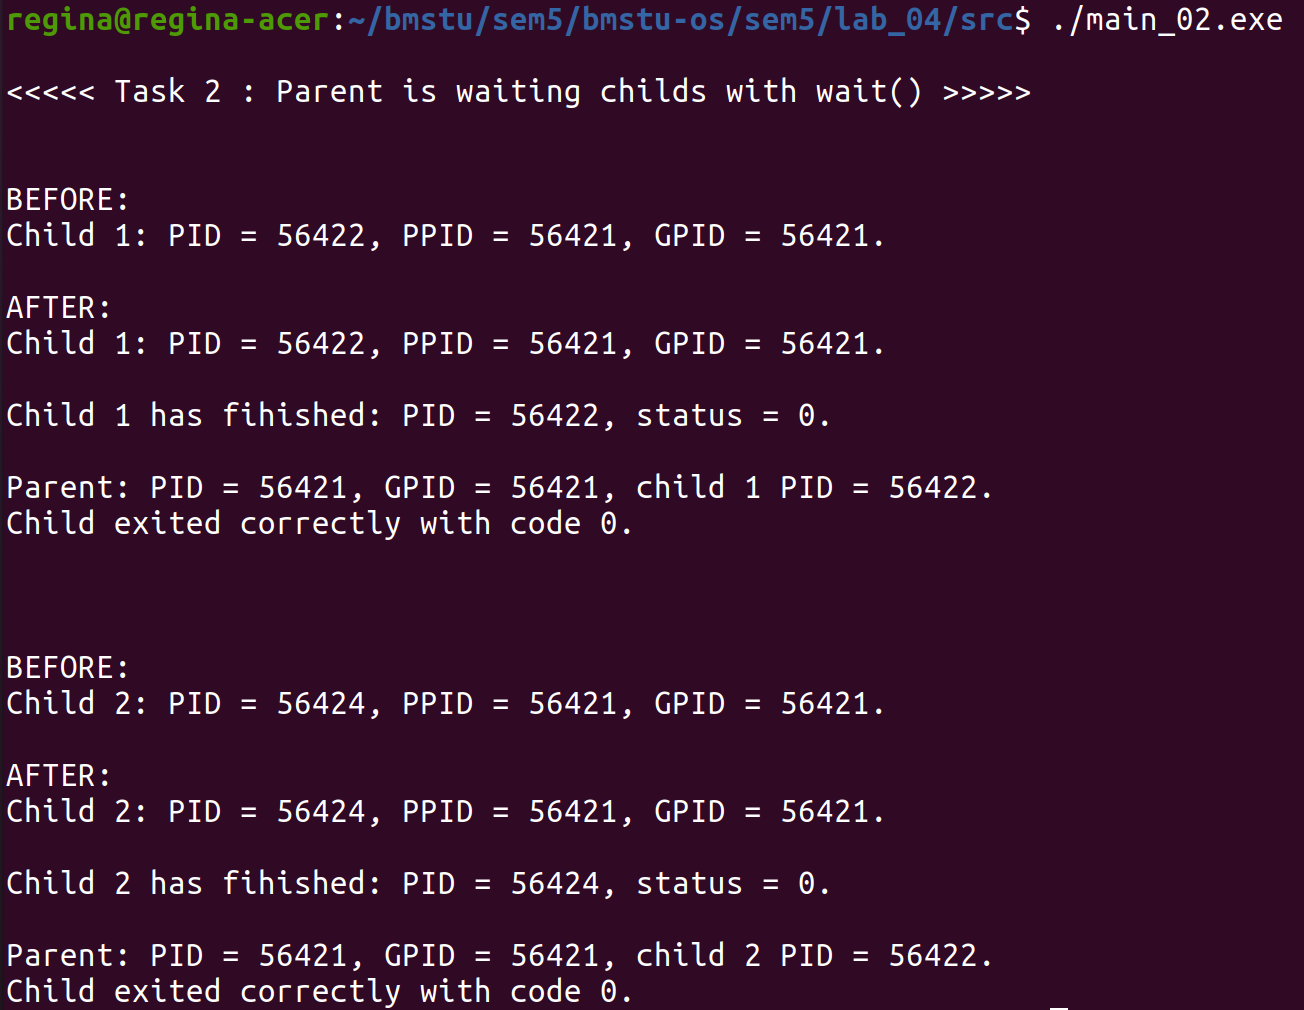
\includegraphics[scale=0.3]{inc/wait.png}
	\end{center}
	\captionsetup{justification=centering}
	\caption{Демонстрация работы программы}
	\label{img:wait}
\end{figure}

\section*{Задание 3}

Процессы-потомки переходят на выполнение следующих программ:

\begin{itemize}
	\item в первой программе (./sort.exe) выполняется чтение массива целых чисел из файла (array.txt), сортировка массива и его вывод на экран (лабораторная работа по курсу программирования на языке C);
	\item во второй программе (./palindrome.exe) выполняется чтение последовательности символов из файла (./string) и вывод сообщения о том, является ли введенная последовательность палиндромом (лабораторная работа по курсу программирования на языке C).
\end{itemize}

Программы передаются системному вызову execlp() в качестве параметра.

\begin{center}
    \captionsetup{justification=raggedright,singlelinecheck=off}
    \begin{lstlisting}[label=lst:exec,caption=Системный вызов execlp]
#include <stdio.h>
#include <stdlib.h>
#include <sys/types.h>
#include <sys/wait.h>
#include <unistd.h>

#define FORK_ERROR -1
#define EXEC_ERROR -1
#define ERROR       1
#define OK          0

#define TASK        "\n<<<<< Task 3 : Children do other programs with execlp() >>>>>\n\n"


void check_status(int status)
{
    if (WIFEXITED(status))
    {
        printf("Child exited correctly with code %d.\n", WEXITSTATUS(status));

        return;
    }
    else if (WIFSIGNALED(status))
    {
        printf("Child exited with non-interceptable signal %d.\n", WTERMSIG(status));

        return;
    }
    else if (WIFSTOPPED(status))
    {
        printf("Child stopped with signal %d.\n", WSTOPSIG(status));

        return;
    }
}


int main(void)
{
    printf(TASK);

    pid_t child_pid1, child_pid2, child_pid;
    int status;

    if ((child_pid1 = fork()) == FORK_ERROR)
    {
        perror("\nCan't fork child 1.\n");
        exit(ERROR);
    }
    else if (child_pid1 == 0)
    {
        printf("\nChild 1 START: PID = %d, PPID = %d, GPID = %d.\n", getpid(), getppid(), getpgrp());
        printf("\n- to sort array\n");

        if (execlp("./sort.exe", "./sort.exe", "array.txt", NULL) == EXEC_ERROR)
        {
            printf("\nERROR: child 1 can not execute exec().\n");

            exit(ERROR);
        }

        exit(OK);
    }
    else
    {
        child_pid = wait(&status);
        printf("\nChild 1 END: PID = %d, status = %d.\n", child_pid, status);

        printf("\nParent: PID = %d, GPID = %d, child 1 PID = %d.\n", getpid(), getpgrp(), child_pid1);
        check_status(status);
    }


    if ((child_pid2 = fork()) == FORK_ERROR)
    {
        perror("\nCan't fork child 2.\n");
        exit(ERROR);
    }
    else if (child_pid2 == 0)
    {
        printf("\n\n\nChild 2 START: PID = %d, PPID = %d, GPID = %d.\n", getpid(), getppid(), getpgrp());
        printf("\n- to check string is palindrome\n");

        if (execlp("./palindrome.exe", "./palindrome.exe", "string.txt", NULL) == EXEC_ERROR)
        {
            printf("\nERROR: child 2 can not execute exec().\n");

            exit(ERROR);
        }

        exit(OK);
    }
    else
    {
        child_pid = wait(&status);
        printf("\nChild 2 END: PID = %d, status = %d\n", child_pid, status);

        printf("\nParent: PID = %d, GPID = %d, child 2 PID = %d\n", getpid(), getpgrp(), child_pid1);
        check_status(status);
    }

    return OK;
}
\end{lstlisting}
\end{center}

\begin{figure}[H]
	\begin{center}
		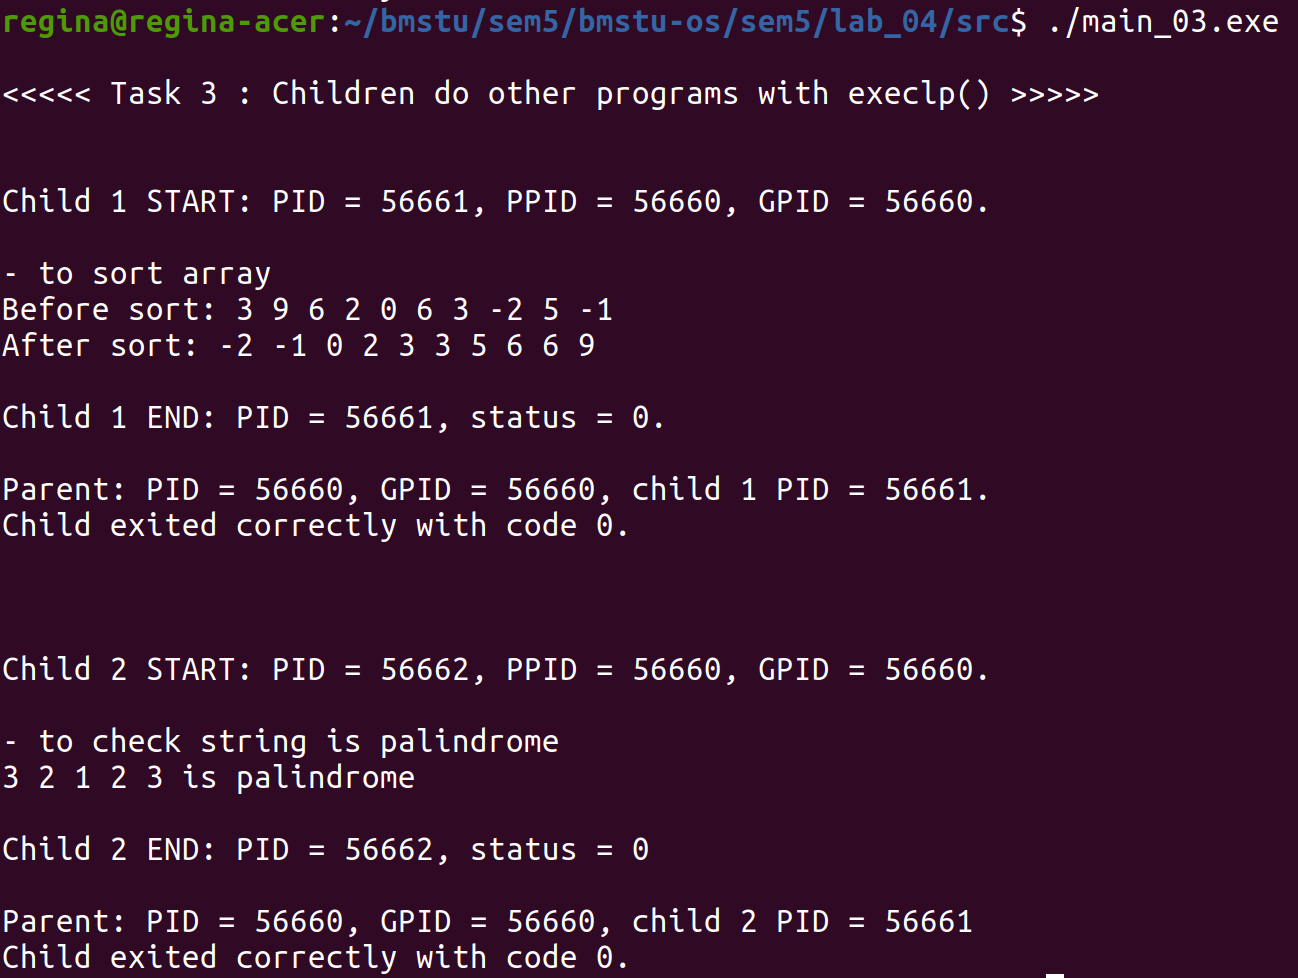
\includegraphics[scale=0.3]{inc/exec.png}
	\end{center}
	\captionsetup{justification=centering}
	\caption{Демонстрация работы программы}
	\label{img:exec}
\end{figure}

\section*{Задание 4}

Процессы-потомки пишут разные сообщения в один неименованный программный канал, созданный системным вызовом pipe(). Процесс-предок считывает сообщения процессов-потомков и выводит сообщения на экран.
\clearpage
\begin{center}
    \captionsetup{justification=raggedright,singlelinecheck=off}
    \begin{lstlisting}[label=lst:pipe,caption=Системный вызов pipe()]
#include <stdio.h>
#include <stdlib.h>
#include <sys/types.h>
#include <sys/wait.h>
#include <unistd.h>
#include <string.h>

#define FORK_ERROR -1
#define PIPE_ERROR -1
#define ERROR       1
#define OK          0


#define TASK        "\n<<<<< Task 4 : Messaging with pipe() >>>>>\n\n"

#define READ  0
#define WRITE 1

#define MSG1  "Hello, child 2.\n"
#define MSG2  "How are you, child 1?\n"
#define LEN   50


void check_status(int status)
{
    if (WIFEXITED(status))
    {
        printf("Child exited correctly with code %d.\n", WEXITSTATUS(status));

        return;
    }
    else if (WIFSIGNALED(status))
    {
        printf("Child exited with non-interceptable signal %d.\n", WTERMSIG(status));

        return;
    }
    else if (WIFSTOPPED(status))
    {
        printf("Child stopped with signal %d.\n", WSTOPSIG(status));

        return;
    }
}

int main(void)
{
    printf(TASK);

    int fd[2];

    pid_t child_pid1, child_pid2, child_pid;
    int status;

    char msgs[LEN] = {0};

    if (pipe(fd) == PIPE_ERROR)
    {
        perror("\nCan't pipe.\n");
        exit(ERROR);
    }

    if ((child_pid1 = fork()) == FORK_ERROR)
    {
        perror("\nCan't fork child 1.\n");
        exit(ERROR);
    }
    else if (child_pid1 == 0)
    {
        printf("\nChild 1: PID = %d, PPID = %d, GPID = %d.\n", getpid(), getppid(), getpgrp());

        close(fd[READ]);
        write(fd[WRITE], MSG1, strlen(MSG1));

        exit(OK);
    }


    if ((child_pid2 = fork()) == FORK_ERROR)
    {
        perror("\nCan't fork child 2.\n");
        exit(ERROR);
    }
    else if (child_pid2 == 0)
    {
        printf("Child 2: PID = %d, PPID = %d, GPID = %d.\n", getpid(), getppid(), getpgrp());

        close(fd[READ]);
        write(fd[WRITE], MSG2, strlen(MSG2));

        exit(OK);
    }

    child_pid = wait(&status);
    printf("\n\nChild 1 has fihished: PID = %d, status = %d.\n", child_pid, status);
    check_status(status);

    child_pid = wait(&status);
    printf("\nChild 2 has fihished: PID = %d, status = %d.\n", child_pid, status);
    check_status(status);

    close(fd[WRITE]);
    read(fd[READ], msgs, LEN);
    printf("\nChilds wrote :\n%s\n", msgs);

    return OK;
}
\end{lstlisting}
\end{center}

\begin{figure}[H]
	\begin{center}
		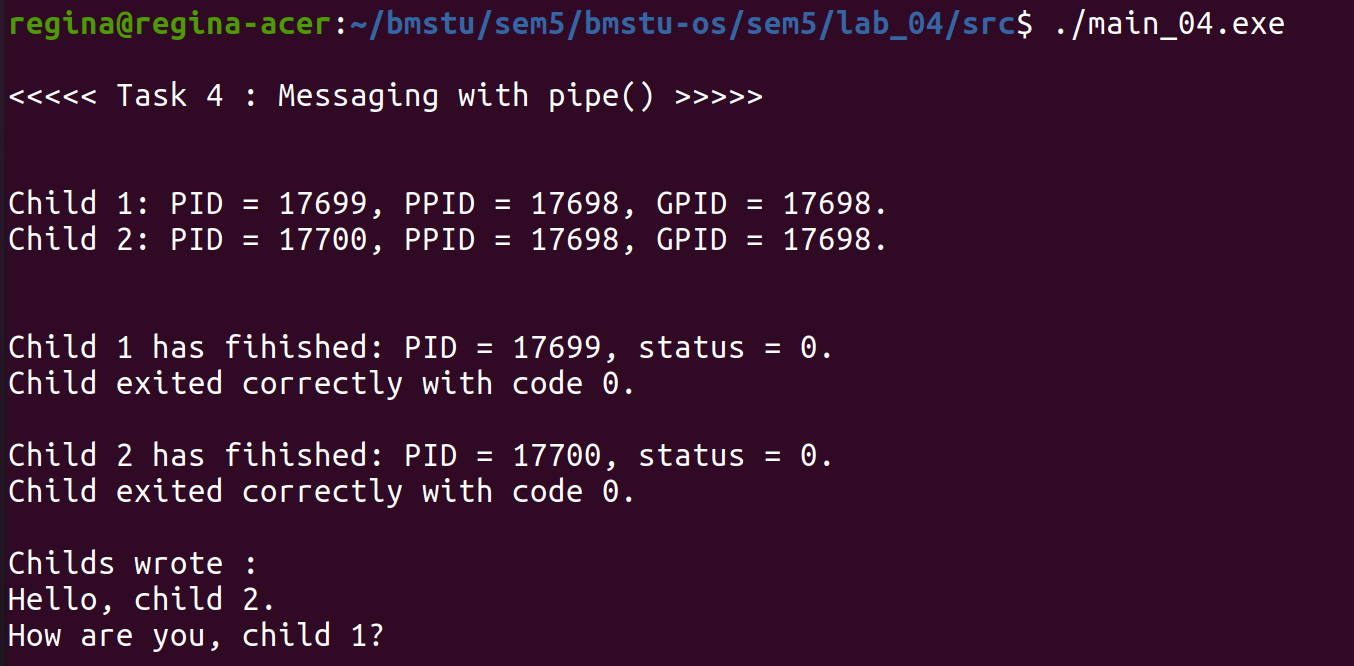
\includegraphics[scale=0.3]{inc/pipe.png}
	\end{center}
	\captionsetup{justification=centering}
	\caption{Демонстрация работы программы}
	\label{img:pipe}
\end{figure}

\section*{Задание 5}

Процесс-предок и процессы-потомки обмениваются сообщениями аналогично заданию 4. При помощи сигнала меняется ход выполнения программы: при получении сигнала от нажатия Ctrl + Z первый процесс-потомок записывает сообщение в канал, при получении сигнала от нажатия Ctrl + C второй процесс-потомок записывает сообщение в канал.

\begin{center}
    \captionsetup{justification=raggedright,singlelinecheck=off}
    \begin{lstlisting}[label=lst:signal,caption=Системный вызов signal()]
#include <stdio.h>
#include <stdlib.h>
#include <sys/types.h>
#include <sys/wait.h>
#include <unistd.h>
#include <string.h>
#include <signal.h>

#define FORK_ERROR -1
#define PIPE_ERROR -1
#define ERROR       1
#define OK          0

#define PAUSE       5

#define TASK        "\n<<<<< Task 5 : Signal handler with signal() >>>>>\n\n"

#define READ  0
#define WRITE 1

#define MSG1  "Hello, child 2.\n"
#define MSG2  "How are you, child 1?\n"
#define LEN   50

#define TRUE   1
#define FALSE  0

#define SIGNAL_MSG "\nPress: CTRL + Z - for msgs from childs\n"


int flag = FALSE;


void check_status(int status)
{
    if (WIFEXITED(status))
    {
        printf("Child exited correctly with code %d.\n", WEXITSTATUS(status));

        return;
    }
    else if (WIFSIGNALED(status))
    {
        printf("Child exited with non-interceptable signal %d.\n", WTERMSIG(status));

        return;
    }
    else if (WIFSTOPPED(status))
    {
        printf("Child stopped with signal %d.\n", WSTOPSIG(status));

        return;
    }
}


void catch_ctrlz(int signal)
{
    flag = TRUE;
    printf("\nCatched signal = %d.\n", signal);
}


int main(void)
{
    printf(TASK);
    printf(SIGNAL_MSG);

    signal(SIGTSTP, catch_ctrlz);
    sleep(PAUSE);

    int fd[2];

    pid_t child_pid1, child_pid2, child_pid;
    int status;

    char msgs[LEN] = {0};

    if (pipe(fd) == PIPE_ERROR)
    {
        perror("\nCan't pipe.\n");
        exit(ERROR);
    }


    if ((child_pid1 = fork()) == FORK_ERROR)
    {
        perror("\nCan't fork child 1.\n");
        exit(ERROR);
    }
    else if (child_pid1 == 0)
    {
        printf("\nChild 1: PID = %d, PPID = %d, GPID = %d.\n", getpid(), getppid(), getpgrp());

        if (flag == TRUE)
        {
            close(fd[READ]);
            write(fd[WRITE], MSG1, strlen(MSG1));
        }

        exit(OK);
    }


    if ((child_pid2 = fork()) == FORK_ERROR)
    {
        perror("\nCan't fork child 2.\n");
        exit(ERROR);
    }
    else if (child_pid2 == 0)
    {
        printf("Child 2: PID = %d, PPID = %d, GPID = %d.\n", getpid(), getppid(), getpgrp());

        if (flag == TRUE)
        {
            close(fd[READ]);
            write(fd[WRITE], MSG2, strlen(MSG2));
        }

        exit(OK);
    }

    child_pid = wait(&status);
    printf("\n\nChild 1 has fihished: PID = %d, status = %d.\n", child_pid, status);
    check_status(status);

    child_pid = wait(&status);
    printf("\nChild 2 has fihished: PID = %d, status = %d.\n", child_pid, status);
    check_status(status);

    close(fd[WRITE]);
    read(fd[READ], msgs, LEN);
    printf("\nChilds wrote :\n%s\n", msgs);

    return OK;
}
\end{lstlisting}
\end{center}

\begin{figure}[H]
	\begin{center}
		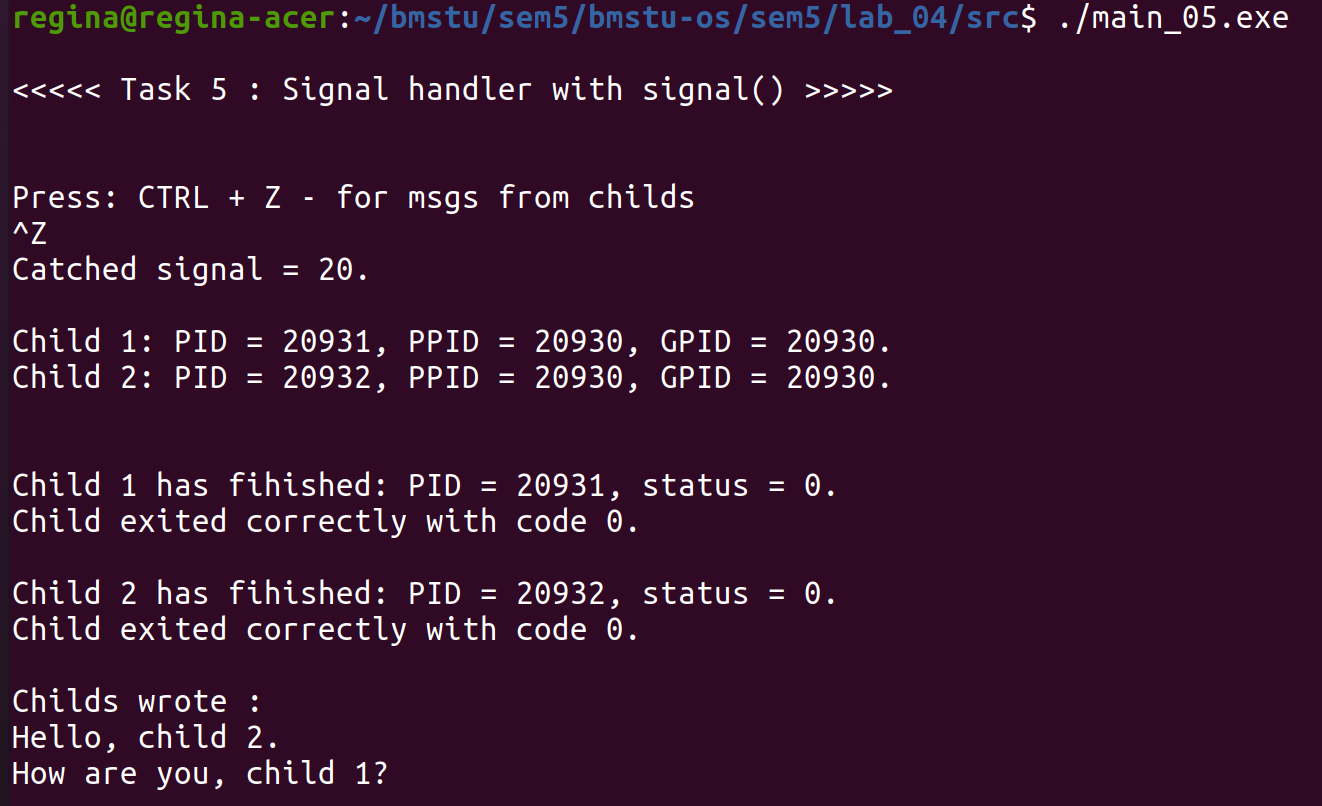
\includegraphics[scale=0.3]{inc/ctrlz.png}
	\end{center}
	\captionsetup{justification=centering}
	\caption{Демонстрация работы программы: сигнал от Ctrl + Z}
	\label{img:ctrlz}
\end{figure}

\begin{figure}[H]
	\begin{center}
		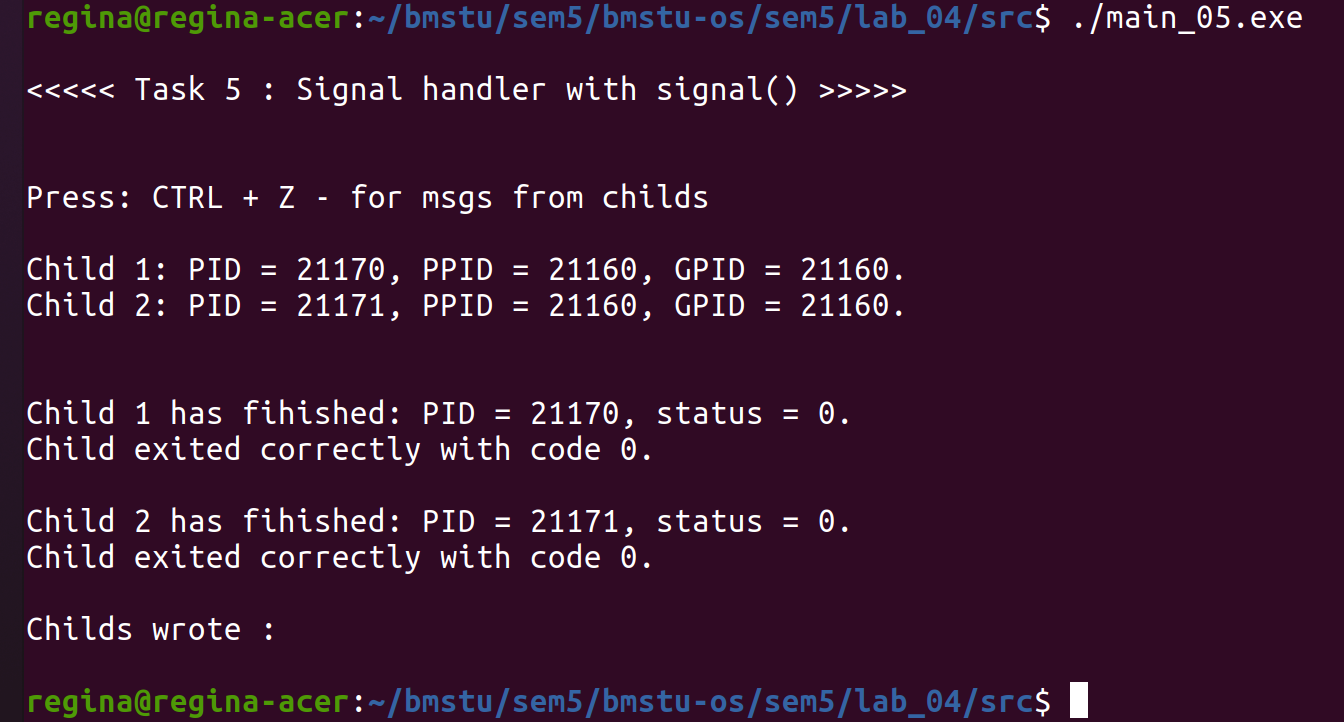
\includegraphics[scale=0.3]{inc/no.png}
	\end{center}
	\captionsetup{justification=centering}
	\caption{Демонстрация работы программы: сигнал не вызван}
	\label{img:no}
\end{figure}

\section*{Последовательность действий при вызове fork()}

\begin{figure}[H]
	\begin{center}
		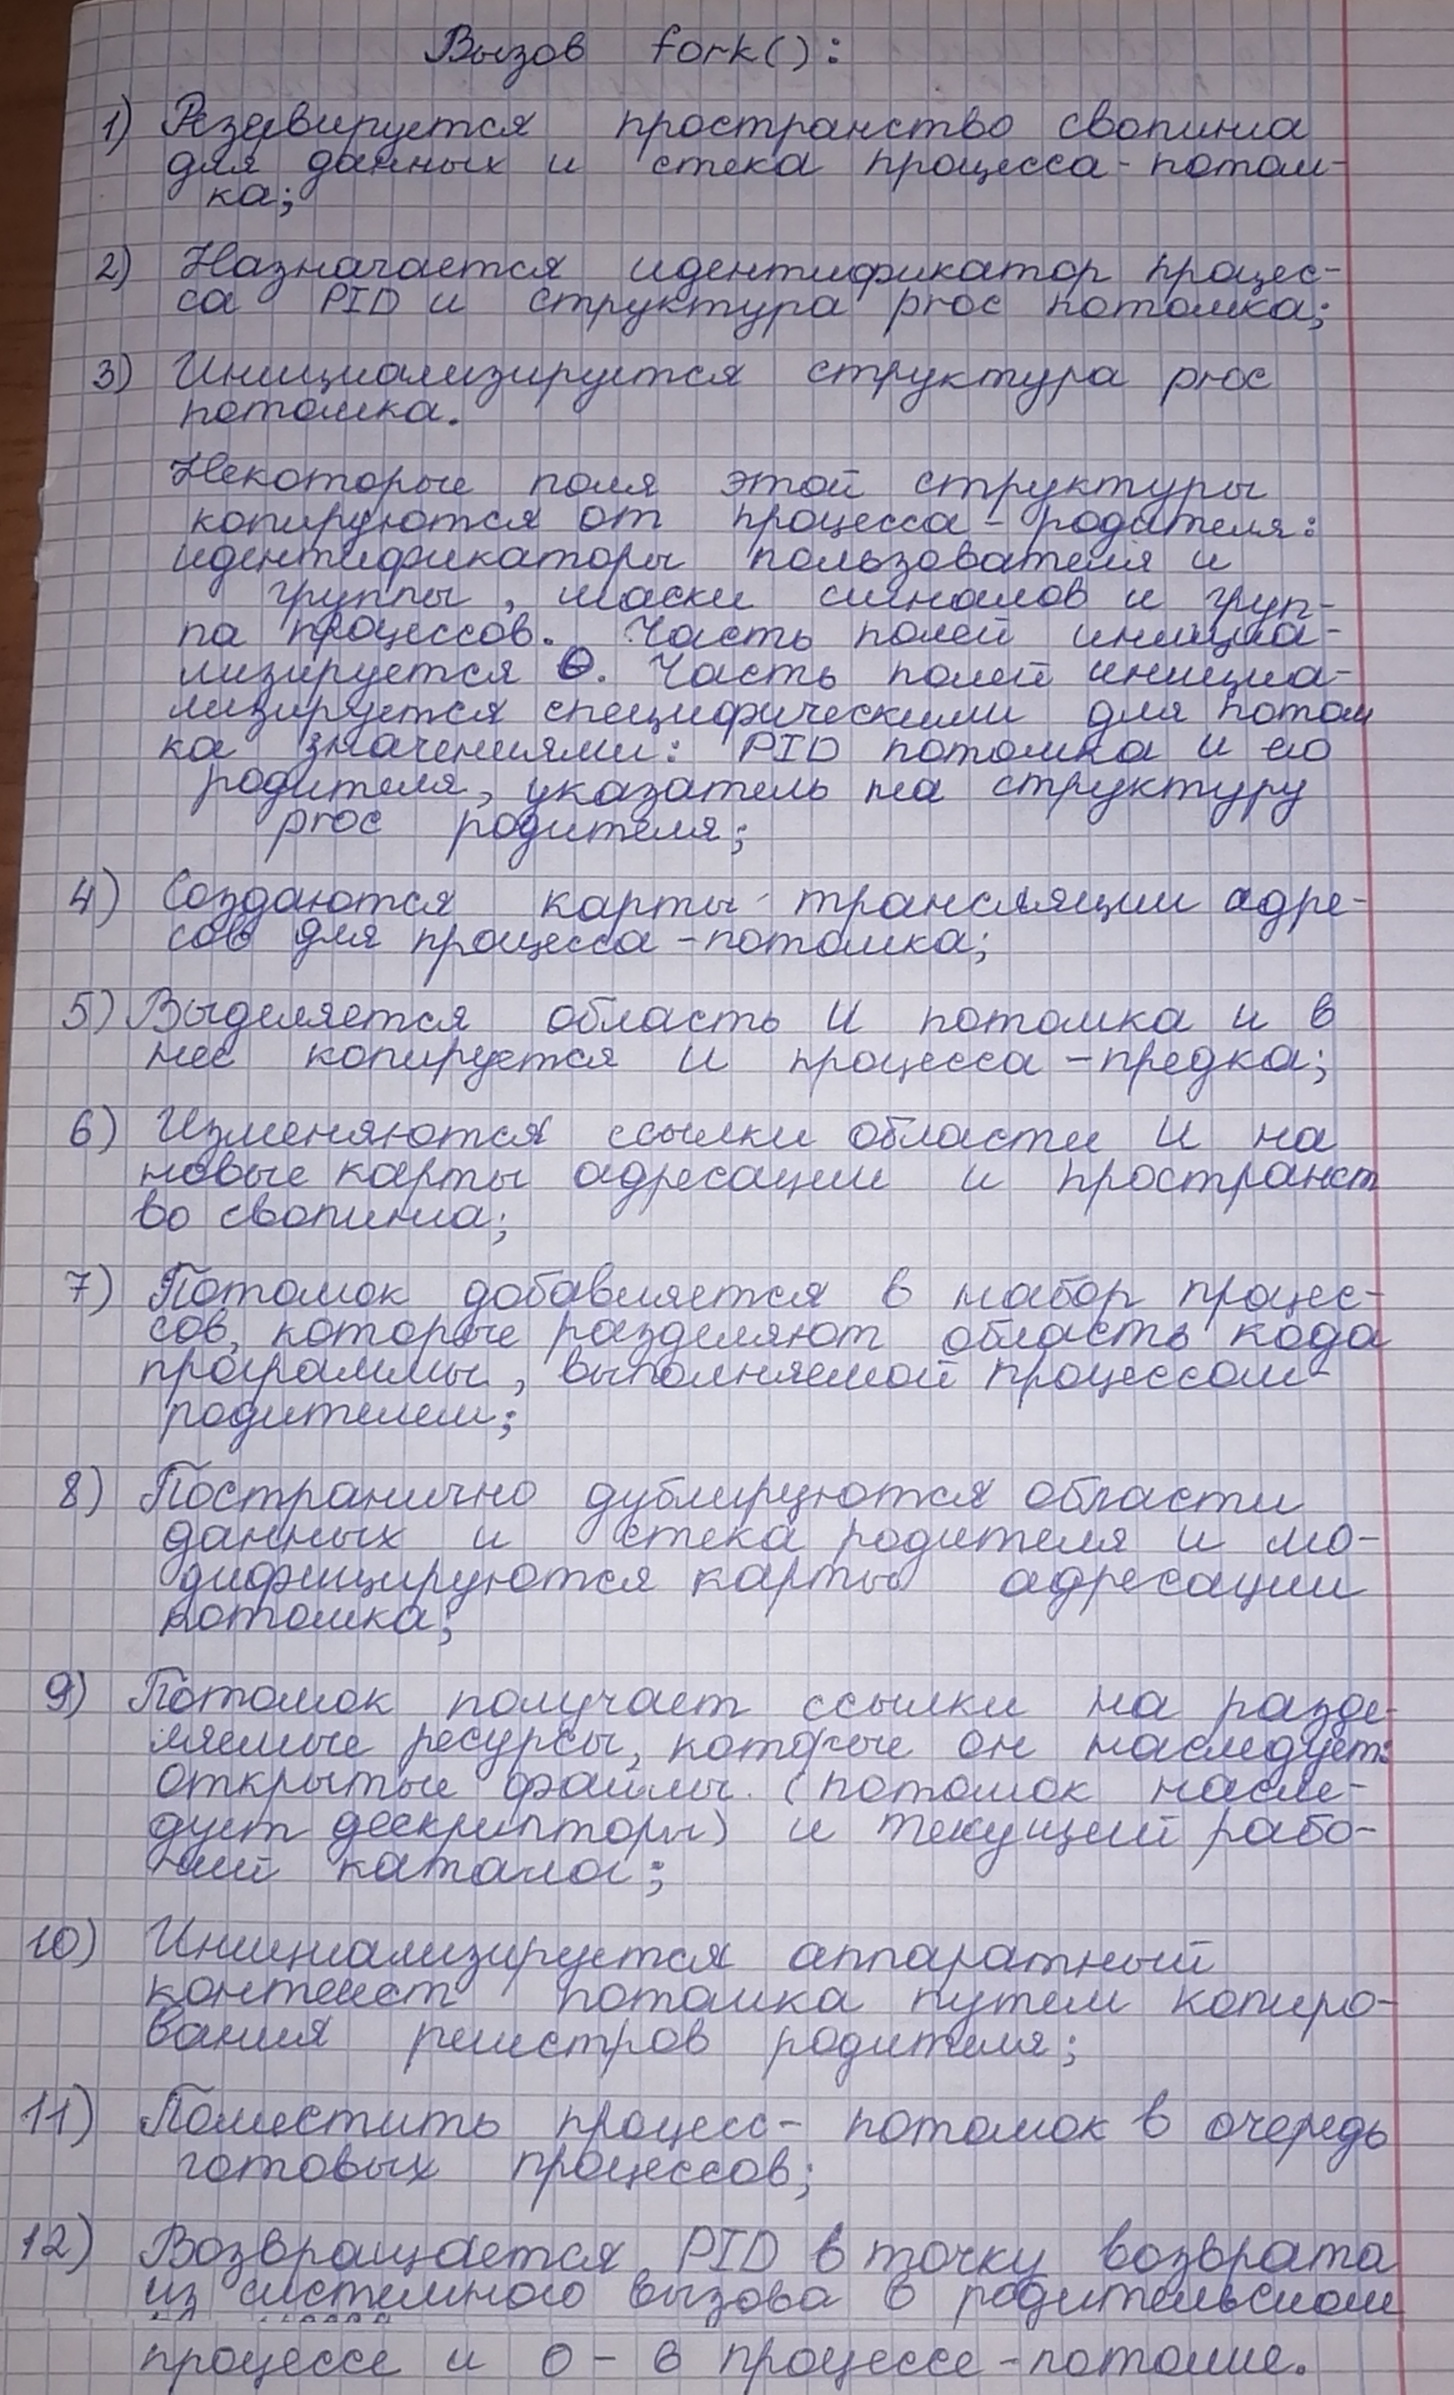
\includegraphics[scale=0.2]{inc/fork.jpg}
	\end{center}
	\captionsetup{justification=centering}
	\caption{Вызов fork()}
	\label{img:fork}
\end{figure}

\section*{Последовательность действий при вызове exec()}

\begin{figure}[H]
	\begin{center}
		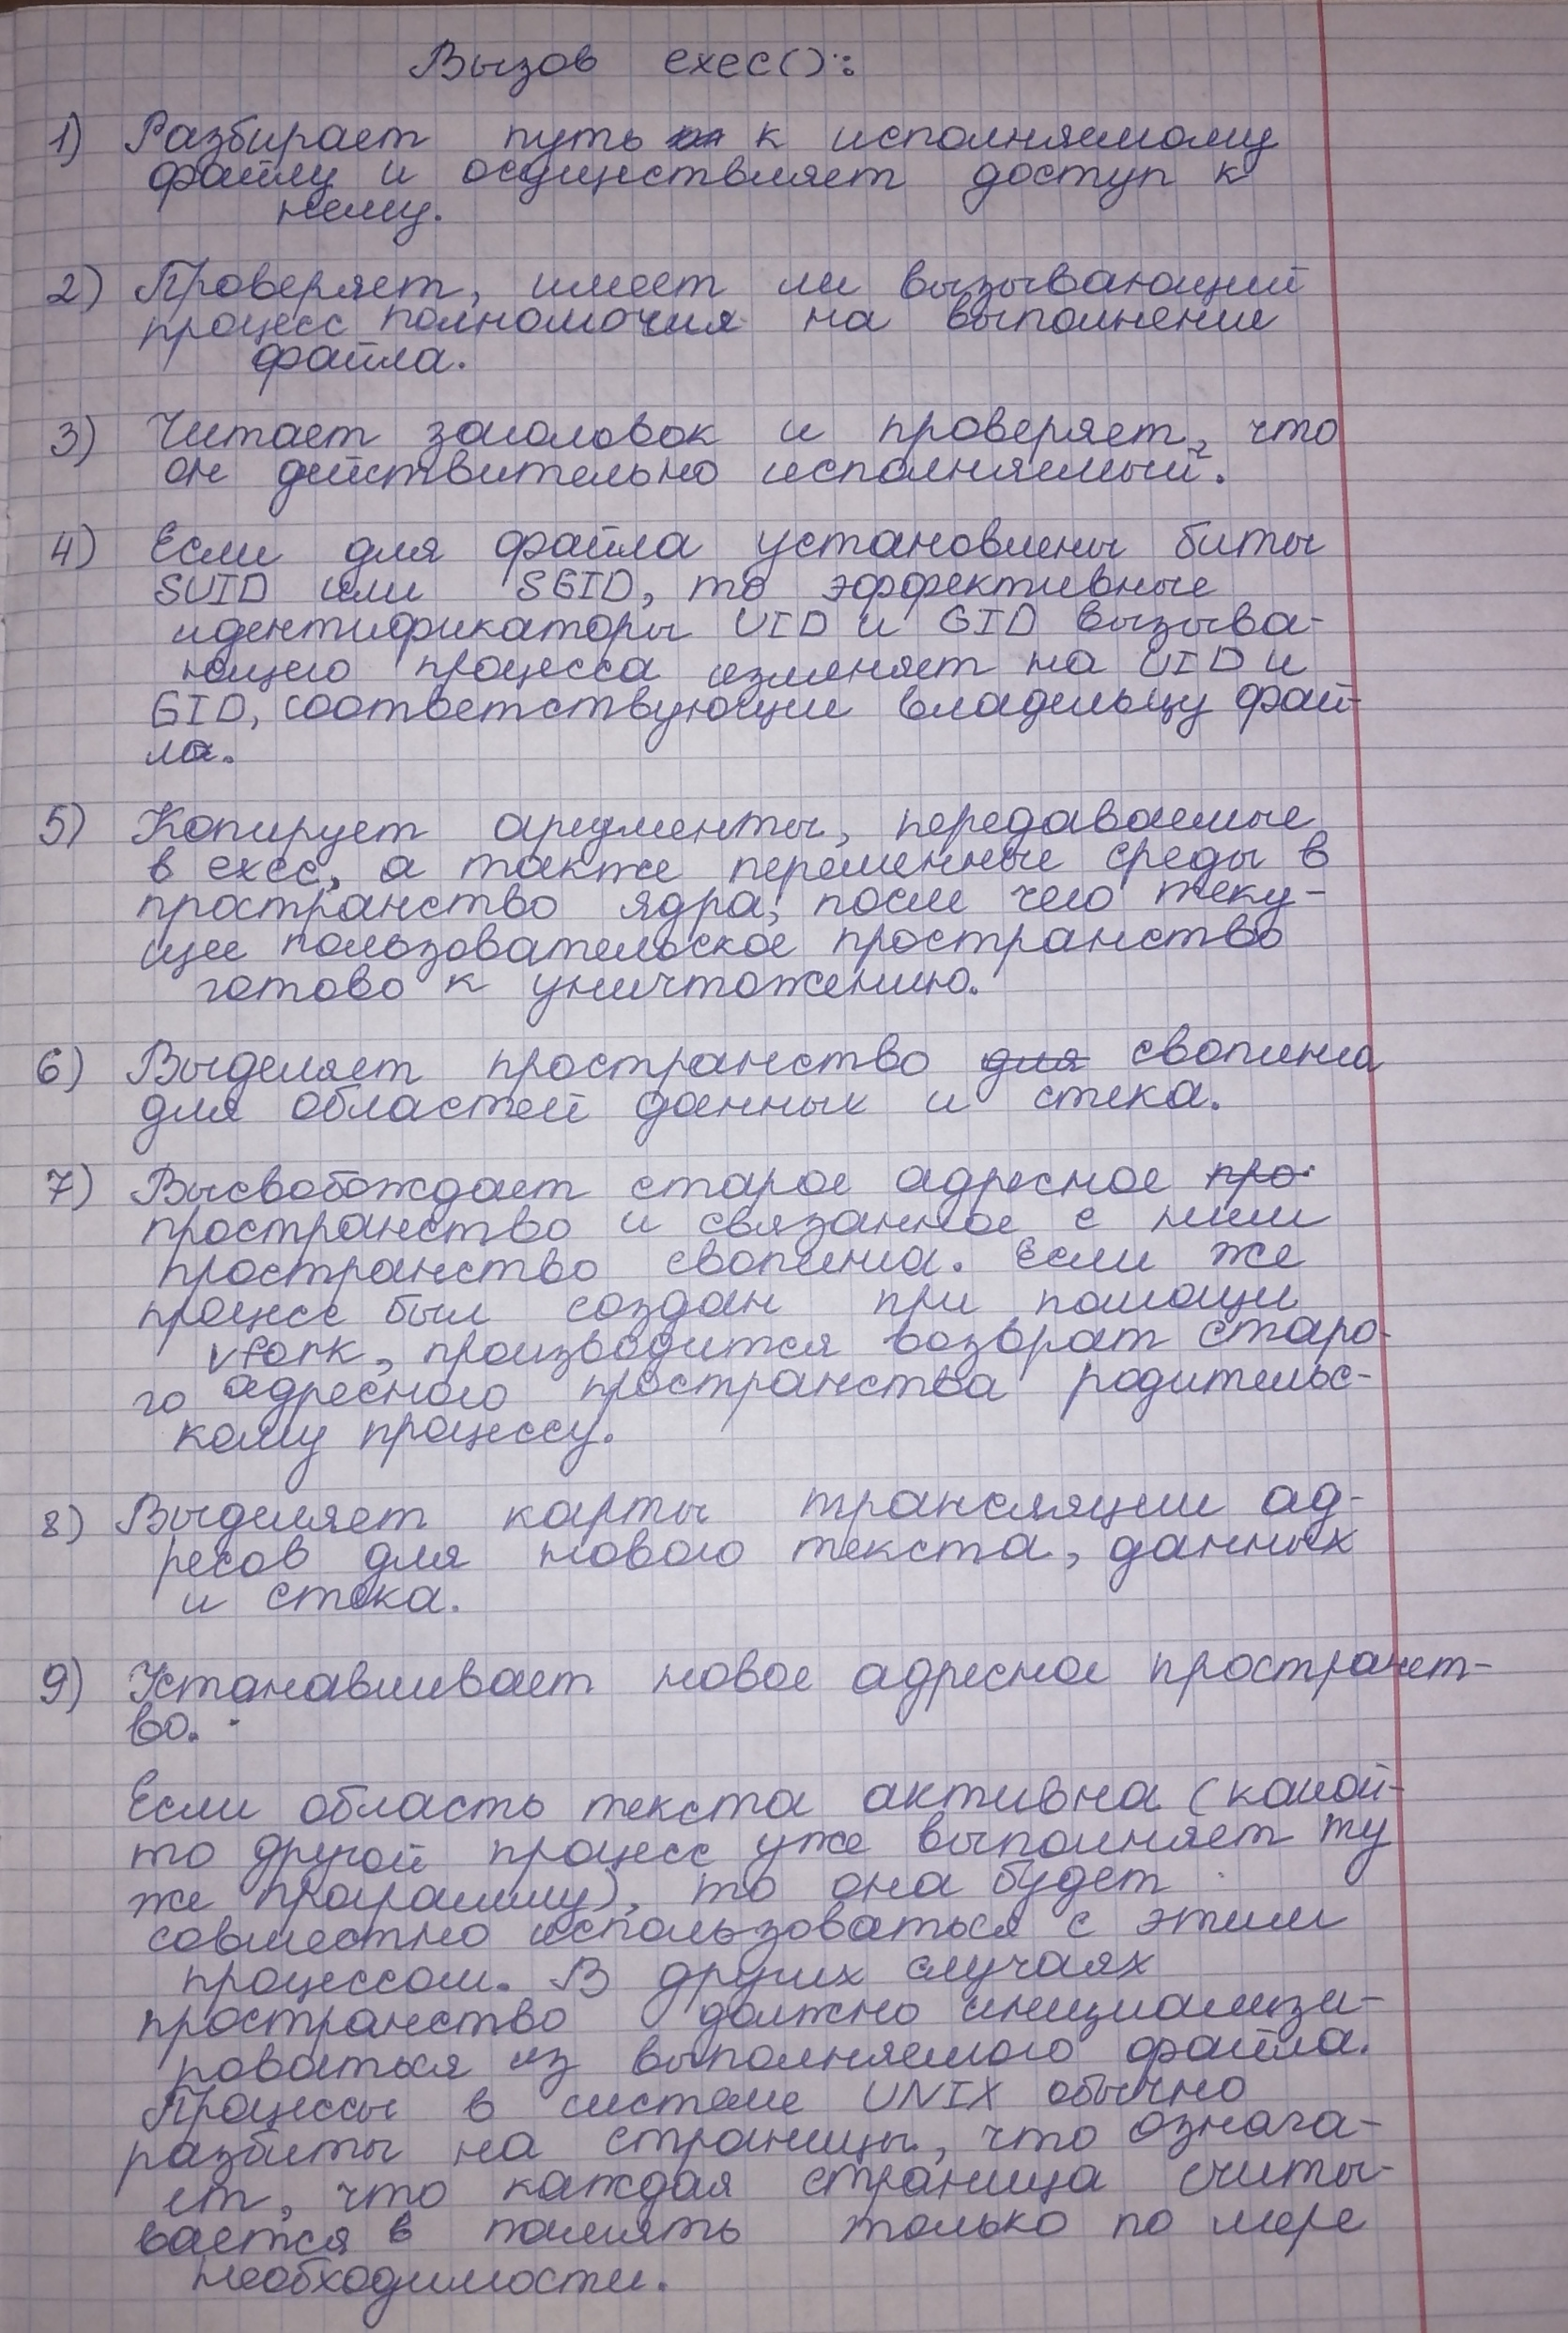
\includegraphics[scale=0.2]{inc/exec1.jpg}
	\end{center}
	\captionsetup{justification=centering}
	\caption{Вызов exec() - 1}
	\label{img:exec1}
\end{figure}

\begin{figure}[H]
	\begin{center}
		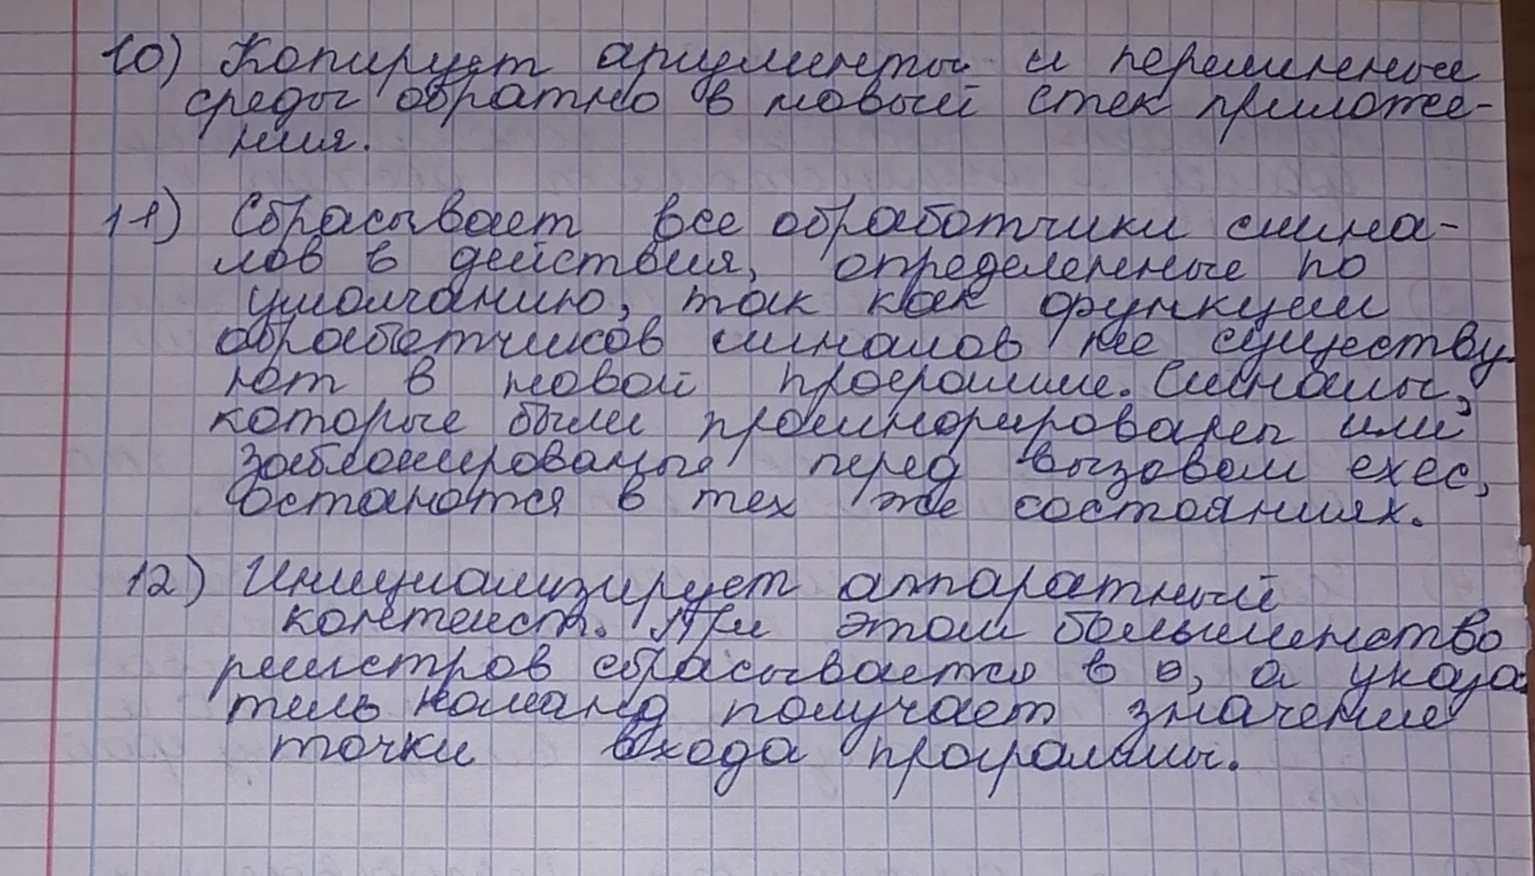
\includegraphics[scale=0.3]{inc/exec2.jpg}
	\end{center}
	\captionsetup{justification=centering}
	\caption{Вызов exec() - 2}
	\label{img:exec2}
\end{figure}